\documentclass[../../main.tex]{subfiles}

\begin{document}
We now focus on the prior probability of the total alternate allele count being $\sigma$ at the locus under consideration: $P(\sum_j g_{ij}=\sigma)=P(\sigma)$. The majority of sites will not include a somatic SNV (sSNV); we say that any site has a prior probability $\lambda$ of having a somatic SNV, which is set to 0.0001 by default~\cite{monovar, sciphi}. %This is for SNPs, accurate for SNVs? Does it matter? SciPHI says no. Perhaps tune hyperparameter from real data.
%
%NB truncal comes from metastatic prostate Gundem et al. NOT strictly true i.e. clonal SNV or SNP(!) with LOH in tree? %TODO : include case of truncal SNV but somatic LOH!
\begin{equation} \label{eq:overallprior}
P(\sigma)=P(\sigma\mid\text{sSNV})\lambda+P(\sigma\mid\neg\text{sSNV})(1-\lambda)
\end{equation}
Any given sample of single cells will only represent some subtree of a full cell phylogeny. As such, when considering the case where there is a sSNV at the locus we can further break down the prior into the case where the sSNV is ancestral to all sampled cells and the case where where the SNV occurs within the subtree rooted at the most recent common ancestor (MRCA) of the cells sampled. We denote the case where the mutation occurs within this subtree as $\text{SNV}_T$.
\begin{equation} \label{eq:somaticsnv}
P(\sigma\mid\text{sSNV})=P(\sigma\mid \text{SNV}_T)P(\text{SNV}_T\mid \text{sSNV})+P(\sigma\mid \text{sSNV},\,\neg\text{SNV}_T)(1-P(\text{SNV}_T\mid \text{sSNV}))
\end{equation}
\subsubsection*{Ploidy changes}
It is well known that many tumor cells may exhibit aneuploidy or chromosomal abnormaities~\cite{gao2016punctuated,21breasts}. For simplicity, we will disregard polyploidy and focus only on the case where loci become haploid. This sort of mutation can result in lost information regarding SNVs, as a loss of heterozygosity can lead to a locus being read as homozygous~\cite{sciphi}. Note that this is an in vivo effect, distinct from allelic dropout which occurs in vitro during DNA ampification. We will model such occurences as a sudden switch to homozygosity, as we cannot reliably distinguish diplod homozygosity from haploidy in the genomic SCS data, which already has significantly uneven coverage and depth~\cite{scprimer}. Let $H$ be the event that the locus under examination has become haploid, and $H_T$ be the case that this mutation has occured within subtree rooted at the MRCA of all sequenced cells.
\begin{equation}
P(\sigma \mid \text{SNV}_T) = P(\sigma\mid\text{SNV}_T,H)P(H) + P(\sigma\mid\text{SNV}_T,\neg H)(1-P(H)) 
\end{equation}
%TODO no prior on P(H). Set as same as lambda? No, in most cancers seems like almost half have CNAs (Gao et al). Also todo remove "initially" from next sentence if don't reestimate
We initially set the value of $P(H)$ to .09 (See Appendix A). In the simplest case, we consider the prior probability of an alternate allele count of $\sigma$ given a mutation occured within the subtree and the locus remained diploid across all sampled cells. Assuming infinite sites, in such a scenario mutations would only be heterozygous.
\begin{equation*}
P(\sigma\mid\text{SNV}_T,\neg H) = \begin{cases} \frac{2m-1}{2(m-1)} T(m,\sigma) \qquad 0<\sigma< m\\ 0 \qquad \qquad \quad \text{else}\end{cases}
\end{equation*}
Where $T(m,\sigma)$ is the prior developed by Singer, Kuipers et al. that assumes a mutation may occur on any branch of the sampled subtree with equal probability.
\begin{equation}\label{eq:T}
T(a,b)=\frac{\binom{a}{b}^2}{(2b-1)\binom{2a}{2b}}
\end{equation}
Now let us consider the case where both a sSNV and a haploid event have both occured at a locus. Since the haploid mutation may have occured in the subtree or ancestral to the subtree, we model these cases seperately.
\begin{equation*}
P(\sigma\mid\text{SNV}_T,H) = P(\sigma\mid\text{SNV}_T,H_T)P(H_T\mid H) + P(\sigma\mid\text{SNV}_T,H,\neg H_T)(1-P(H_T\mid H)) \label{eq:SNVT}
\end{equation*}
\subsubsection*{SNV and loss of heterozygosity within the subtree}
In the first scenario described by Equation~\ref{eq:SNVT} both a point mutation and a ploidy change have occured within the sequenced subtree. This can be split into four further subcases (Figure~\ref{fig:treecases}).

\begin{figure}[h]\label{fig:treecases}
	\centering

	\begin{subfigure}{0.2\textwidth}
		\centering
		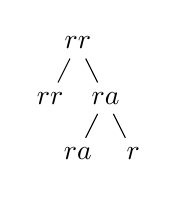
\begin{tikzpicture}[sibling distance=2em, level distance=2em]
  \node {$rr$}
    child { node {$rr$} }
    child { node {$ra$}
      child { node {$ra$} }
      child { node {$r$}}
          };
		\end{tikzpicture}
		\caption{Case 1}
	\end{subfigure}
	\begin{subfigure}{0.2\textwidth}
		\centering
		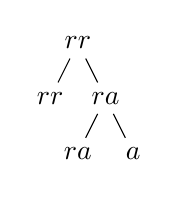
\begin{tikzpicture}[sibling distance=2em, level distance=2em]
  \node {$rr$}
    child { node {$rr$} }
    child { node {$ra$}
      child { node {$ra$} }
      child { node {$a$}}
          };
		\end{tikzpicture}
		\caption{Case 2}
	\end{subfigure}
	\begin{subfigure}{0.2\textwidth}
		\centering
		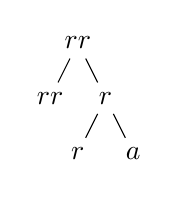
\begin{tikzpicture}[sibling distance=2em, level distance=2em]
  \node {$rr$}
    child { node {$rr$} }
    child { node {$r$}
      child { node {$r$} }
      child { node {$a$}}
          };
		\end{tikzpicture}
		\caption{Case 3}
	\end{subfigure}
	\begin{subfigure}{0.2\textwidth}
		\centering
		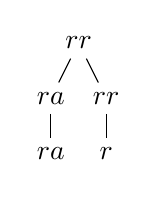
\begin{tikzpicture}[sibling distance=2em, level distance=2em]
  \node {$rr$}
    child { node {$ra$} 
    	child { node {$ra$} }
    	  }
    child { node {$rr$} 
    	child { node {$r$} }
    	};
		\end{tikzpicture}
		\caption{Case 4}
	\end{subfigure}
	
	\caption{SNV and haploid event both within the subtree. (a) Point mutation happens before haploid event and mutated allele is dropped. (b) Point mutation happens before haploid event and reference allele is dropped. (c) Haploid event occurs before point mutation. Since haploid cells are modelled as becoming homozygous diploids, this case leads to only even values of alternate allele count. (d) In this case the point mutation and haploid event do not occur in the same lineage. We ignore this case as the haploid event does not affect the alternate allele count.}
\end{figure}
Considering the above three cases where a ploidy change in the subtree affects the locus alternate allele count, it is twice as likely that the point mutation should occur before the haploid event (cases 1 and 2), compared with the other temporal ordring (case 3). Therefore $P(\text{case 1 or 2})=2/3$ and $P(\text{case 3})=1/3$. This is because the cells before a haploid event, being diploid, have twice the chance of having a point mutation at a locus than the haploid descendants of such a mutation. We also assume the refence and alternate alleles have an equal chance of being dropped in a loss of heterozygosity.
\begin{equation*}
P(\text{case 1})=P(\text{case 2}) = P(\text{case 3}) = 1/3
\end{equation*}
Continuing to assume that both a point mutation and a haploid event have occured within the sequenced subtree at the locus in question, we now have
\begin{equation*}
P(\sigma\mid\text{SNV}_T,H_T)=\frac{1}{3}\left[P(\sigma\mid\text{case 1})+P(\sigma\mid\text{case 2})+P(\sigma\mid\text{case 3})\right]
\end{equation*}
%TODO nb only one value of h is applicable for each a
%TODO this means h is somewhat cumbersome notation. Better to substitute h = a-sigma
To examine these probabilities we will use the function $T(a,b)$ described above, which given a subtree with $a$ leaves gives the probability of a mutation affecting $b$ of those leaves. For case 1, the loss of heterozygosity effectively deletes all alternate alleles from the cells sharing a lineage with the haploid event, and so
\begin{equation*}
P(\sigma\mid\text{case 1}) = \frac{2m-1}{2(m-1)}\sum_{a-h=\sigma}T(m,a)T(a,h)\qquad 1\leq a < m,\;1\leq h\leq a
\end{equation*}
%TODO : Very slow computation!!
While we include one normalization constant, excluding the case of an ancestral point mutation, we do allow the case where a point mutation and a loss of heterozygosity happen on the same branch of the phylogeny. Hence the support for $\sigma$ in case 1 is $[0,m)$. Since we model a haploid event as a sudden switch to homozygosity, the observed allele count for case 2 is the number of cells affected by the heterozygous point mutation ($a$) added to the number of cells affected by the loss of heterozygosity ($h$).
\begin{equation*}
P(\sigma\mid\text{case 2}) = \frac{2m-1}{2(m-1)}\sum_{a+h=\sigma}T(m,a)T(a,h) \qquad 1\leq a < m,\;1\leq h\leq a
\end{equation*}
For case 2, the support is [2,\,2m-2]. In case 3, only even allele counts can be produced as all cells carrying the point mutation are haploid, which we model as being homozygous mutated. The possible values of $\sigma$ are $1\leq\sigma\leq 2m-2$.
\begin{equation*}
P(\sigma\mid\text{case 3}) = \frac{2m-1}{2(m-1)}\sum_{2a=\sigma} T(m,h)T(h,a) \qquad 1\leq h < m,\; h\geq a
\end{equation*}
\subsubsection*{Haploid subtree}
Referreing back to Equation~\eqref{eq:SNVT}, we must determine the prior probability of an alternate allele count $\sigma$ at a locus given that a point mutation occured within the sequenced subtree and a haploid event occured ancestral to the subtree. This would lead to all sampled cells being haploid at this locus, therefore allowing only even allele counts.
\begin{equation*}
P(\sigma\mid \text{SNV}_T,H,\neg H_T) = \begin{cases} \frac{2m-1}{2(m-1)}T(m,\frac{\sigma}{2})\qquad 2\mid\sigma,\;0<\sigma<2m\\ 0 \qquad\qquad\qquad\quad \text{else} \end{cases}
\end{equation*}
\subsubsection*{Clonal and subclonal mutations}
We have so far considered the case where sSNVs have been subclonal: they may affect some of our sampled cells and not others. There is some probability however that a sSNV at a given locus may be due to a mutation in a cell ancestral to all sampled cells. The majority of these ancestral mutations will affect all tumour cells: so-called clonal, truncal or public mutations~\cite{neutralevoltumour, 21breasts, metastatic}. If the sample of single cells is small enough, however, it could be the case that a subclonal mutation is common to all cells sampled.
\begin{equation}
P(\text{ancestral}\mid \text{sSNV})=P(\text{clonal})+P(\text{ancestral}\mid \text{subclonal})(1-P(\text{clonal}))
\end{equation}
To find the probability of a subclonal mutation affecting all sampled cells, we assume tumour subclones follow a neutral evolutionary model such that subclonal mutant allele frequencies follow a power law distribution~\cite{neutralevoltumour}. Using an IID model for tumour cell sampling, the probability that all $m$ cells are from a subclone with cellular frequency $2f$ (allelic frequency = $f$) is $(2f)^m$. Similar to Williams et al. we define a probability density function for the allelic frequency of subclonal mutations proportional to the inverse of the allelic frequency.\\
%TODO how can assume heterozygosity??)
\begin{equation}
P(f) = k\left(\frac{1}{f}-2\right)
\end{equation}
where $k$ is a normalization constant. We define the support of $P(f)$ for subclones as $[10^{-8},0.5]$, as a frequency of $10^{-8}$ is on the order of affecting single cells and an allelic frequency of $0.5$ corresponds to clonal mutations~\cite{numcells}. We find a value of $k$ by integrating $P(f)$ over this support. If a subclonal mutation affects all sampled cells, then all these cells must be from the same subclone.
\begin{equation} \label{eq:tmids}
P(\text{ancestral}\mid \text{subclonal}) = \int_f P(\text{all in subclone}\mid f)P(f)\,df=\int_{10^{-8}}^{0.5}(2f)^mk\left(\frac{1}{f}-2\right)\,df
\end{equation}
For large enough samples ($m>30$) the probability that all cells were sampled from a single subclone (Equation~\ref{eq:tmids}) becomes negligible. Since it is only a function of $m$ these values are pre-computed for efficiency. The empirically estimated probability that any given mutation is clonal is set at $P(\text{clonal})=0.51$ (see appendix A)~\cite{21breasts, metastatic, yachida}. Having developed the probability that any given somatic mutation is ancestral to all sampled cells, we have also found the probability that a mutation has occured within the sampled subtree.
\begin{equation*}
P(\text{SNV}_T\mid\text{sSNV})=P(H_T\mid H)=1-P(\text{ancestral}\mid\text{sSNV})
\end{equation*}

\subsubsection*{Ancestral sSNVs}
Referring Equation~\eqref{eq:somaticsnv} we must also determine the prior for $\sigma$ in the case that the sSNV is ancestral to all cells. Without LOH this would always result in $\sigma=m$, however we must again consider haploid events both within and ancestral to the sampled subtree.
\begin{equation} \label{eq:ancestralsnv}
P(\sigma\mid\text{sSNV},\,\neg\text{SNV}_T)=P(\sigma\mid\text{sSNV},\,\neg\text{SNV}_T,\,H)P(H)+P(\sigma\mid\text{sSNV},\,\neg\text{SNV}_T,\,\neg H)(1-P(H))
\end{equation}
If there is no haploid event, there will be no LOH and the ancestral sSNV will be heterozygous across all cells.
\begin{equation*}
P(\sigma\mid\text{sSNV},\,\neg\text{SNV}_T,\,\neg H) = \begin{cases}1\quad \sigma=m\\ 0\quad\text{else}\end{cases}
\end{equation*}
In the case of a haploid event, we must consider the cases where the whole subtree is haploid and when the haploid event happens within the subtree. We also consider the alternate and reference alleles to be dropped with equal probability as above.
\begin{align*}
P(\sigma\mid\text{sSNV},\,\neg\text{SNV}_T,\,H)=&(1-P(H_T\mid H))P(\sigma\mid \text{sSNV},\,\neg\text{SNV}_T,\,H,\,\neg H_T)\\
&+P(H_T\mid H)P(\sigma\mid H_T,\,\text{SNV},\,\neg\text{SNV}_T)
\end{align*}
If both the somatic SNV and the haploid event are ancestral to the sequenced subtree, the cells will either all be haploid reference or all be haploid alternate with equal probability. Since we model haploid cells as homozygous diploid this results in only alternate allele counts of $0$ or $2m$.
\begin{equation*}
P(\sigma\mid\text{sSNV},\,\neg\text{SNV}_T,\,H,\,\neg H_T)= \begin{cases} \frac{1}{2} \quad \sigma=0,2m\\0\quad \text{else} \end{cases}
\end{equation*}
If there is an sSNV ancestral to the sampled cells but a haploid event occured within the sampled subtree we may have any alternate allele count from $1$ to $2m-1$ depending on where in the phylogeny heterozygosity was lost and which allele was dropped.
\begin{equation*}
P(\sigma\mid\text{sSNV},\,\neg\text{SNV}_T,\,H_T) = \begin{cases} \frac{1}{2}T(m,\sigma-m)\qquad \sigma > m\\
\frac{1}{2}T(m,m-\sigma)\qquad m > \sigma \end{cases}
\end{equation*}

\end{document}
